%%%%%%%%%%%%%%%%%%%%%%%%%%%%%%%%%%%%%%%%%%%%%%%%%%%%%%%%%%%%%%%%%%%%%%%%%%%%%%%%%%%%%%%%%%%%%%%%%%%
%
%   Máster Universitario en Ciencia de Datos (MUCD) 
%   Template for APPSIV labs
%   Author: Álvaro García Martín
%
%   THIS TEMPLATE IS READING ONLY!!!
%   TO EDIT THIS TEMPLATE, LOG IN OVERLEAF AND COPY THIS TEMPLATE
%   
%%%%%%%%%%%%%%%%%%%%%%%%%%%%%%%%%%%%%%%%%%%%%%%%%%%%%%%%%%%%%%%%%%%%%%%%%%%%%%%%%%%%%%%%%%%%%%%%%%%
\documentclass[letterpaper, 10 pt, conference]{ieeeconf}  

% The following packages can be found on http:\\www.ctan.org
\usepackage{graphicx} % for pdf, bitmapped graphics files
%\usepackage{epsfig} % for postscript graphics files
\usepackage{mathptmx} % assumes new font selection scheme installed
\usepackage{times} % assumes new font selection scheme installed
\usepackage{amsmath} % assumes amsmath package installed
\usepackage{amssymb}  % assumes amsmath package installed
\usepackage{xcolor}
\usepackage{float}
\usepackage{minted}
\usepackage{hyperref}


\usepackage{tikz}
\usetikzlibrary{shapes.geometric}

\hypersetup{
    colorlinks=true,
    linkcolor=blue,
    filecolor=magenta,
    citecolor = black,
    urlcolor=cyan,
    pdftitle={Overleaf Example},
    pdfpagemode=FullScreen,
    }

\newcommand{\E}{\mathbb E}
\newcommand{\PP}{\text{P}}

\def\inline{\lstinline[basicstyle=\ttfamily,keywordstyle={}]}


\usepackage{caption}
\usepackage{subcaption}


\usepackage{biblatex}
\addbibresource{bibliography.bib}

\title{\LARGE \bf  (Not really) achieving state-of-art classification accuracy in video classification}

\author{Álvarez J. Sáez J.}

\begin{document}

\maketitle
\thispagestyle{headings}
\pagestyle{headings}

%%%%%%%%%%%%%%%%%%%%%%%%%%%%%%%%%%%%%%%%%%%%%%%%%%%%%%%%%%%%%%%%%%%%%%%%%%%%%%%%
\section{INTRODUCTION}

It is known that the supervised image classification problem is getting close to be completely solved \cite{COCA}. The developed models are becoming more complex and powerful, being able to obtain very good representations that lead to models with incredible performance.

Videos are concatenations in the time axis- of numerous images, where it is common that the image in time \(t\) is related to images \(t-1\) and \(t+1\), and probably also related to further steps of time. With this consideration, it is natural to extend the techniques used in single images to videos in order perform different tasks. 

In this practical assignment, we consider the video classification task. In this task, given a set of videos \(\mathcal X\) labeled by \textbf{actions performed in this video} \(\mathcal Y\), we aim to find a function \(f: \mathcal X \to \mathcal Y\) that tells which action is performed in each video of our set \(\mathcal X\). This is also known as the \textbf{action recognition task}.

To achieve this, we will test a few different methods: a fixed class one, a random class one, and a CNN frame-by-frame model. We will present a theoretical analysis of the error of the first two methods and then explain how we executed the third method and the results obtained. We obtain very high accuracy scores when using the frame-by-frame method. These accuracy scores decrease when we increase the number of classes.

The rest of this report is structures as follows: section \ref{section:method} briefly describes the implemented methods, chapter \ref{section:implementation} discusses implementation details, chapter \ref{section:data} describes the dataset used, chapter \ref{section:results} details our models results and the respective analysis, chapter \ref{section:conclusions} presents our final conclusions and chapter \ref{section:timelog} describes the time log followed for this assignment.

%NOTE: section titles are tentative, you may change them to fit your needs. It is suggested to include figures and tables in the report.
%%%%%%%%%%%%%%%%%%%%%%%%%%%%%%%%%%%%%%%%%%%%%%%%%%%%%%%%%%%%%%%%%%%%%%%%%%%%%%%%
\section{METHODOLOGY}
\label{section:method}

In this section we briefly describe the video classification models implemented for this practical assignment and develop a theorical analysis for the results expected by two of them.

Let us stablish a simple notation for our theorical study. Let $M$ be the number of classes in our dataset and let $X \{(x_i, c_i), \ i = 1,\dots, N \}$ our dataset, where $c_i$ is the class associated to sample $i$. Our guess for the $i-$sample will be $\hat c_i$, chosen differently depending on the method. Our main metric will be the \textbf{accuracy}:

\[
    \textbf{Acc} = \E \left[ \PP \left [ c_i = \hat c_i \right ] \right ].
\]

Finally, let $|C_j|$ be the number of elements in the $j-$th class, for $j \in \{1, \ldots, M\}$. Since every sample has a single associated class we also know that

\begin{equation}
    \label{eq:classes}
    \sum_{j=1}^M |C_j| = N.
\end{equation}

\subsection{Method 1: Fixed class}

The first model implemented is quite simple: a single class is fixed beforehand, and the model predicts that class for every sample. Let us study the expected accuracy for the method.

Let $m \in \{1, \ldots, N\}$ be our fixed class. Then $\hat c_i = m$ for every sample. The accuracy can be expressed as follows

\[
    \textbf{Exp Acc} = \E \left[ \PP \left [ c_i = m \right ] \right ].
\]

If the dataset was balanced (there were the same number of samples in every class), the probability of element $c_i$ being in class $m$ would be $1/M$:

\[
    \textbf{Exp Acc}_\text{bal} = \E \left[ \PP \left [ c_i = m \right ] \right ]  = \E \left[ \frac{1}{M} \right ] = \frac{1}{M}.
\]

However, this is not always the case. For instance the dataset used in this practical assignment, \textbf{UCF101}, is not balanced, as we will see in section \ref{section:data}. In this case, the probability of the $i-$th sample being in class $m$ is the ratio of elements in the $m$ class in our dataset:

\[
    \textbf{Exp Acc}_\text{inbal} = \E \left[ \PP \left [ c_i = m \right ] \right ]  = \E \left[ \frac{|C_m|}{N} \right ] = \frac{|C_m|}{N}.
\]

Finally, the inbalanced case must generalize the balanced one. If the data was balance, the number of elements in the $m$ class would be $N/M$, and the balanced and inbalanced accuracies match:

\[
    \textbf{Exp Acc}_\text{inbal} = \frac{|C_m|}{N} = \frac{N/M}{N} = \frac{1}{M} = \textbf{Exp Acc}_\text{bal}.
\]

\subsection{Method 2: Random choice}

The second model is not much more complicated: for every video the model predicts a class chosen uniformly at random. Let us study the expected accuracy for the method.

In this case, our prediction $\hat c_j$ is uniformly randomly pick from the set \{1, \ldots, M\}. The accuracy can be computed directly:

\begin{align*}
    \textbf{Exp Acc} & = \E \left[ \PP \left [ \hat c_i = c_i \right ] \right ] \\
    & = \E \left[ \sum_{m=1}^M \PP \left[ \hat c_i = m \right] \PP \left[ c_i = m \right] \right] \\
    & = \E \left[ \sum_{m=1}^M \frac{1}{M} \frac{|C_m|}{N} \right] \\
    & = \E \left[ \frac{1}{MN} \sum_{m=1}^M |C_m| \right] \\
    & \substack{(1) \\ =} \; \E \left[ \frac{1}{MN} \cdot N \right] \\
    & = \frac{1}{M} \\
\end{align*}

where in $(1)$ we used equation \ref{eq:classes}. As we can see, the way of selecting a random class for each sample makes the expected accturacy stable so it doesn't depend on the number of classes. If we were to choose between this and the previous method without previously knowing the distributions of classes in the dataset, the second algorithm would be more consistent.

\subsection{Method 3: CNN}

This method is the first method that is not completely doomy. As we mentioned in the introduction, videos are concatenations of images so a very good idea is to treat them as splitted images. 

In this assignment, we will use the frame-by-frame paradigm. In particular, we will use the framework proposed in \cite{CNN}. 


\begin{figure}[H]
\small
\centering
\hspace{-0.4in}
\resizebox{0.85\linewidth}{!}{%
\makeatletter
\pgfkeys{/pgf/.cd,
  parallelepiped offset x/.initial=2mm,
  parallelepiped offset y/.initial=2mm
}
\pgfdeclareshape{parallelepiped}
{
  \inheritsavedanchors[from=rectangle] % this is nearly a rectangle
  \inheritanchorborder[from=rectangle]
  \inheritanchor[from=rectangle]{north}
  \inheritanchor[from=rectangle]{north west}
  \inheritanchor[from=rectangle]{north east}
  \inheritanchor[from=rectangle]{center}
  \inheritanchor[from=rectangle]{west}
  \inheritanchor[from=rectangle]{east}
  \inheritanchor[from=rectangle]{mid}
  \inheritanchor[from=rectangle]{mid west}
  \inheritanchor[from=rectangle]{mid east}
  \inheritanchor[from=rectangle]{base}
  \inheritanchor[from=rectangle]{base west}
  \inheritanchor[from=rectangle]{base east}
  \inheritanchor[from=rectangle]{south}
  \inheritanchor[from=rectangle]{south west}
  \inheritanchor[from=rectangle]{south east}
  \backgroundpath{
    % store lower right in xa/ya and upper right in xb/yb
    \southwest \pgf@xa=\pgf@x \pgf@ya=\pgf@y
    \northeast \pgf@xb=\pgf@x \pgf@yb=\pgf@y
    \pgfmathsetlength\pgfutil@tempdima{\pgfkeysvalueof{/pgf/parallelepiped
offset x}}
    \pgfmathsetlength\pgfutil@tempdimb{\pgfkeysvalueof{/pgf/parallelepiped
offset y}}
    \def\ppd@offset{\pgfpoint{\pgfutil@tempdima}{\pgfutil@tempdimb}}
    \pgfpathmoveto{\pgfqpoint{\pgf@xa}{\pgf@ya}}
    \pgfpathlineto{\pgfqpoint{\pgf@xb}{\pgf@ya}}
    \pgfpathlineto{\pgfqpoint{\pgf@xb}{\pgf@yb}}
    \pgfpathlineto{\pgfqpoint{\pgf@xa}{\pgf@yb}}
    \pgfpathclose
    \pgfpathmoveto{\pgfqpoint{\pgf@xb}{\pgf@ya}}
    \pgfpathlineto{\pgfpointadd{\pgfpoint{\pgf@xb}{\pgf@ya}}{\ppd@offset}}
    \pgfpathlineto{\pgfpointadd{\pgfpoint{\pgf@xb}{\pgf@yb}}{\ppd@offset}}
    \pgfpathlineto{\pgfpointadd{\pgfpoint{\pgf@xa}{\pgf@yb}}{\ppd@offset}}
    \pgfpathlineto{\pgfqpoint{\pgf@xa}{\pgf@yb}}
    \pgfpathmoveto{\pgfqpoint{\pgf@xb}{\pgf@yb}}
    \pgfpathlineto{\pgfpointadd{\pgfpoint{\pgf@xb}{\pgf@yb}}{\ppd@offset}}
  }
}
\makeatother

\ifx\du\undefined
  \newlength{\du}
\fi
\setlength{\du}{1.5\unitlength}
\ifx\spacing\undefined
  \newlength{\spacing}
\fi
\setlength{\spacing}{30\unitlength}
\begin{tikzpicture}
\pgfsetlinewidth{0.7500\du}
\pgfsetmiterjoin
\pgfsetbuttcap

\node[parallelepiped,draw=black,
  minimum width=50\du,minimum height=\du,
  parallelepiped offset x=30\du,
  parallelepiped offset y=20\du] (1a) at (0, -\spacing) {};
  \node[anchor=center] at (0.4\spacing, -0.7\spacing){Frame $t$};

\node[parallelepiped,draw=black, dotted,
  minimum width=30\du,minimum height=\du,
  parallelepiped offset x=20\du,
  parallelepiped offset y=15\du] (2a) at (0, -\spacing) {};

\node[anchor=center] at (0.4\spacing, -0.7\spacing){Frame $t$};



\node[parallelepiped,draw=black,
  minimum width=50\du,minimum height=\du,
  parallelepiped offset x=30\du,
  parallelepiped offset y=20\du] (1b) at (5\spacing, -\spacing) {};
  \node[anchor=center] at (5.4\spacing, -0.7\spacing){Frame $t+1$};

\node[parallelepiped,draw=black, dotted,
  minimum width=30\du,minimum height=\du,
  parallelepiped offset x=20\du,
  parallelepiped offset y=15\du] (2b) at (5\spacing, -\spacing) {};

\node[parallelepiped,draw=black,
  minimum width=50\du,minimum height=\du,
  parallelepiped offset x=30\du,
  parallelepiped offset y=20\du] (1c) at (10\spacing, -\spacing) {};
  \node[anchor=center] at (10.4\spacing, -0.7\spacing){Frame $t+2$};

\node[parallelepiped,draw=black, dotted,
  minimum width=30\du,minimum height=\du,
  parallelepiped offset x=20\du,
  parallelepiped offset y=15\du] (2c) at (10\spacing, -\spacing) {};

\node[rectangle, draw=black, minimum width=10\du, minimum height=40\du] (f1) at (0.3\spacing, 3.0\spacing) {};
\node[rectangle, draw=black, minimum width=10\du, minimum height=40\du] (f2) at (1.3\spacing, 3.0\spacing) {};
\node[rectangle, draw=black, minimum width=10\du, minimum height=40\du] (f3) at (2.3\spacing, 3.0\spacing) {};

\node[rectangle, draw=black, minimum width=10\du, minimum height=40\du] (f4) at (0\spacing, 2.5\spacing) {};
\node[rectangle, draw=black, minimum width=10\du, minimum height=40\du, color=blue] (f5) at (0.9\spacing, 2.5\spacing) {};
\node[rectangle, draw=black, minimum width=10\du, minimum height=40\du, color=red] (f10) at (1.1\spacing, 2.5\spacing) {};
\node[rectangle, draw=black, minimum width=10\du, minimum height=40\du] (f6) at (2\spacing, 2.5\spacing) {};

\node[rectangle, draw=black, minimum width=10\du, minimum height=40\du] (f7) at (-0.3\spacing, 2.0\spacing) {};
\node[rectangle, draw=black, minimum width=10\du, minimum height=40\du] (f8) at (0.7\spacing, 2.0\spacing) {};
\node[rectangle, draw=black, minimum width=10\du, minimum height=40\du] (f9) at (1.7\spacing, 2.0\spacing) {};


\node[rectangle, draw=black, minimum width=10\du, minimum height=40\du] (g1) at (5.3\spacing, 3.0\spacing) {};
\node[rectangle, draw=black, minimum width=10\du, minimum height=40\du] (g2) at (6.3\spacing, 3.0\spacing) {};
\node[rectangle, draw=black, minimum width=10\du, minimum height=40\du] (g3) at (7.3\spacing, 3.0\spacing) {};

\node[rectangle, draw=black, minimum width=10\du, minimum height=40\du] (g4) at (5\spacing, 2.5\spacing) {};
\node[rectangle, draw=black, minimum width=10\du, minimum height=40\du, color=blue] (g5) at (5.9\spacing, 2.5\spacing) {};
\node[rectangle, draw=black, minimum width=10\du, minimum height=40\du, color=red] (g10) at (6.1\spacing, 2.5\spacing) {};
\node[rectangle, draw=black, minimum width=10\du, minimum height=40\du] (g6) at (7\spacing, 2.5\spacing) {};

\node[rectangle, draw=black, minimum width=10\du, minimum height=40\du] (g7) at (4.7\spacing, 2.0\spacing) {};
\node[rectangle, draw=black, minimum width=10\du, minimum height=40\du] (g8) at (5.7\spacing, 2.0\spacing) {};
\node[rectangle, draw=black, minimum width=10\du, minimum height=40\du] (g9) at (6.7\spacing, 2.0\spacing) {};


\node[rectangle, draw=black, minimum width=10\du, minimum height=40\du] (h1) at (10.3\spacing, 3.0\spacing) {};
\node[rectangle, draw=black, minimum width=10\du, minimum height=40\du] (h2) at (11.3\spacing, 3.0\spacing) {};
\node[rectangle, draw=black, minimum width=10\du, minimum height=40\du] (h3) at (12.3\spacing, 3.0\spacing) {};

\node[rectangle, draw=black, minimum width=10\du, minimum height=40\du] (h4) at (10\spacing, 2.5\spacing) {};
\node[rectangle, draw=black, minimum width=10\du, minimum height=40\du, color=blue] (g5) at (10.9\spacing, 2.5\spacing) {};
\node[rectangle, draw=black, minimum width=10\du, minimum height=40\du, color=red] (g10) at (11.1\spacing, 2.5\spacing) {};
\node[rectangle, draw=black, minimum width=10\du, minimum height=40\du] (h6) at (12\spacing, 2.5\spacing) {};

\node[rectangle, draw=black, minimum width=10\du, minimum height=40\du] (h7) at (9.7\spacing, 2.0\spacing) {};
\node[rectangle, draw=black, minimum width=10\du, minimum height=40\du] (h8) at (10.7\spacing, 2.0\spacing) {};
\node[rectangle, draw=black, minimum width=10\du, minimum height=40\du] (h9) at (11.7\spacing, 2.0\spacing) {};


\node[anchor=center] (1ap) at (0.7\spacing, -0.7\spacing){};
\node[anchor=center] (2ap) at (5.7\spacing, -0.7\spacing){};
\node[anchor=center] (3ap) at (10.7\spacing, -0.7\spacing){};
\node[anchor=center] (1aq) at (-1.5\spacing, 1.5\spacing){Frame Patch};
\draw[ultra thick, ->] (1ap) -- (f8);
\draw[ultra thick, ->] (2ap) -- (g8);
\draw[ultra thick, ->] (3ap) -- (h8);
\draw[thick, -] (1aq) -- (1ap);
\node[rectangle, draw=black, minimum width=60\du, minimum height=10\du] (pool) at (6\spacing, 5.5\spacing) {Video level CNN features};

\node[anchor=center] at (2.5\spacing, 0.5\spacing){CNN feature extraction};
\node[anchor=center] at (7.5\spacing, 0.5\spacing){CNN feature extraction};
\node[anchor=center] at (12.5\spacing, 0.5\spacing){CNN feature extraction};
\node[anchor=center] at (10.7\spacing, 4.8\spacing){Spatiotemporal pooling and normalization};
\node[anchor=center] (svm) at (10\spacing, 5.5\spacing){SVM};
\draw[ultra thick, ->] (f2) -- (pool);
\draw[ultra thick, ->] (g2) -- (pool);
\draw[ultra thick, ->] (h2) -- (pool);
\draw[ultra thick, ->] (pool) -- (svm);
\end{tikzpicture}

}
%\\
%\vspace{0.2in}
%\includegraphics[width=0.8\columnwidth]{fig/overview.pdf}
%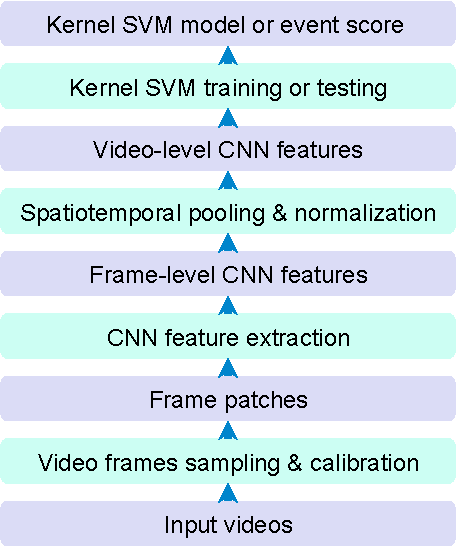
\includegraphics[width=0.23\linewidth]{Figures/overview_v.pdf}
%\vspace{-5 pt}
\caption{Overview of the proposed video classification pipeline.}
\label{fig:overview}
\end{figure}

A brief summary of the framework's workflow is shown in Figure \ref{fig:overview}. The main idea is to split the whole video in different frames and apply a CNN to each of the images and, when the features are extracted, perform an spatiotemporal pooling to summarize the features of all the frames into a single vector that can be classified using any kind of model. This method acheived state-of-the-art results in UCF101 when it was firt presented.

It is important to remark that, in this assignment, the CNN architecture that we use is InceptionV3, which can be automatically loaded from Keras. We substract the last layers and manually add the spatiotemporal pooling and a linear classifier.

In this case, computing the expected accuracy of our model is not straightforward, since it is a neural network \cite{UNCERTAINTY}.


%%%%%%%%%%%%%%%%%%%%%%%%%%%%%%%%%%%%%%%%%%%%%%%%%%%%%%%%%%%%%%%%%%%%%%%%%%%%%%%%
\section{IMPLEMENTATION}
\label{section:implementation}
\subsection{Functions for Methods}

The first two methods are implemented in file \mintinline{bash}{random_vs_fixed_mode.py}. The fixed class for the first method is hardcoded in the file, and the implementation itself is quite straight-forward.

The third model is implemented in file \mintinline{bash}{random_vs_fixed_mode.py}, specifically in the \mintinline{bash}{get_model()} function. We only needed to obtain the InceptionV3 pretrained model without the last top layers, add a global average pooling and a final dense layer.

Additionally, functions \mintinline{bash}{freeze_all_but_top()} and \mintinline{bash}{freeze_all_but_mid_and_top()} were implemented. They freeze every layer but the top two and every layer but the midel and top layers respectively, and are used during training. Firstly, the top two layers are trained with the default learning rate, $0.01$. Secondly, the mid and top layers and trained with a much lower learning rate, $0.0001$, for fine-tuning.

\subsection{Checkpoints}

When it came to executing the experiments of the last model, we struggled executing it for the whole \(100\) epochs. The execution of the training in the file \mintinline{bash}{train_cnn.py} failed after an arbitrary number of epochs (about thirty: sometimes more, sometimes less). The error shown was:

\begin{minted}[fontsize=\footnotesize]{bash}
Error occurred when finalizing GeneratorDataset
iterator: FAILED_PRECONDITION: Python interpreter
state is not initialized.
The process may be terminated.
	 [[{{node PyFunc}}]]
\end{minted}

After a deep search in different forums (such as StackOverflow, Github and Keras documentation), we could not determine the specific reason for this mistake, although we had the suspicion that the error was dued to a difficulty in matching the batch size with the steps per epoch \footnote{According to \href{https://stackoverflow.com/questions/60000573/error-occurred-when-finalizing-generatordataset-iterator-cancelled-operation-w}{this answer} from Stack Overflow  }.\\

We decided to, since everything during the training seemed to be working fine, implement a few functions to be able to resume the training at any point. This way we only would have to reexecute the train script. In order to achieve this, we added the following functionalities:
\begin{itemize}
    \item Changed the folder structure in order to have all the logs of the same model in the same file (a log file is created for each execution of the train script, we merged them all to create the results). The new structure is \mintinline{bash}{data/logs/'class_limit'_'seq_limit'}. Using this, we got our results well split and plotting the results only requires file management.
    \item A new \mintinline{bash}{ModelCheckpoint} that creates a checkpoint every \(10\) epochs.
    \item A function that loads the last checkpoint. This function is called \mintinline{bash}{load_previous_weights} and, briefly, it searches the required weights file matching the number of classes and segment size and loads it (if it exists) and returns the number of executed epochs. Using the number of epochs, the model only trains the remaining epochs up to \(100\).
    \item Lastly, the pipeline for beginning the training is changed a little bit so that we firstly try to load a previous model automatically. Thanks to this, if our script fails, we only have to reexecute the script to continue the training.
\end{itemize}

Thanks to this functionality, we were able to finish this assignment. Otherwise the code could not have been executed.

\subsection{Running the code}
The practical assignment submission consists of two jupyter notebook called \mintinline{bash}{VideoClassification.ipynb} and \mintinline{bash}{plotting.ipynb}, along with a folder called \mintinline{bash}{P2}. The experiments can be reproduced by following step by step the jupyter notebook, although the data and the saved checkpoints are not in the submitted folder.

Along the execution, several checkpoints will be automatically created. As explained in the proevious subsection, the code will automatically load the last saved checkpoint and continue the execution from that point onwards.

After the execution, we can use the obtained logs and the functions from file \mintinline{bash}{plot_utils.py} (adapted from the one given provided for this assignment) to plot this accuracy and loss evolutions. This process is automated in the jupyter notebook \mintinline{bash}{plotting.ipynb}.

Finally, the different arguments and parameters and in the relevant implemented functions. For any changes, see the jupyter notebook or the respective python files.

%%%%%%%%%%%%%%%%%%%%%%%%%%%%%%%%%%%%%%%%%%%%%%%%%%%%%%%%%%%%%%%%%%%%%%%%%%%%%%%%

\section{DATA}
\label{section:data}

In this section, we will describe the used dataset. UCF101 \cite{UCF101} was (when first presented) the largest dataset of human actions. As it name indicates, it consits on \(101\) action classes. In this dataset, we can find over \(13k\) clips and \(27\) hours of video data.

\begin{figure}[H]
    \centering
    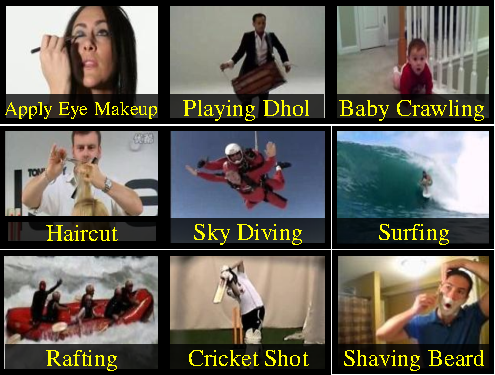
\includegraphics[scale=0.8]{Figures/first_page_v1.pdf}
    \caption{A few examples of labeled actions from the dataset UCF101 \cite{UCF101}.}
    \label{fig:ucf101}
\end{figure}

In the first experiment, we used only the first \(5\) classes of the dataset.  In Figure \ref{fig:hist_5} the histogram of the class distribution is shown. As we can see, these five classes are a little bit imbalanced, which will lead to not exactly uniform results in the random algorithms, as we explained in the theoretical disquisition from section \ref{section:method}.

\begin{figure}[H]
    \centering
    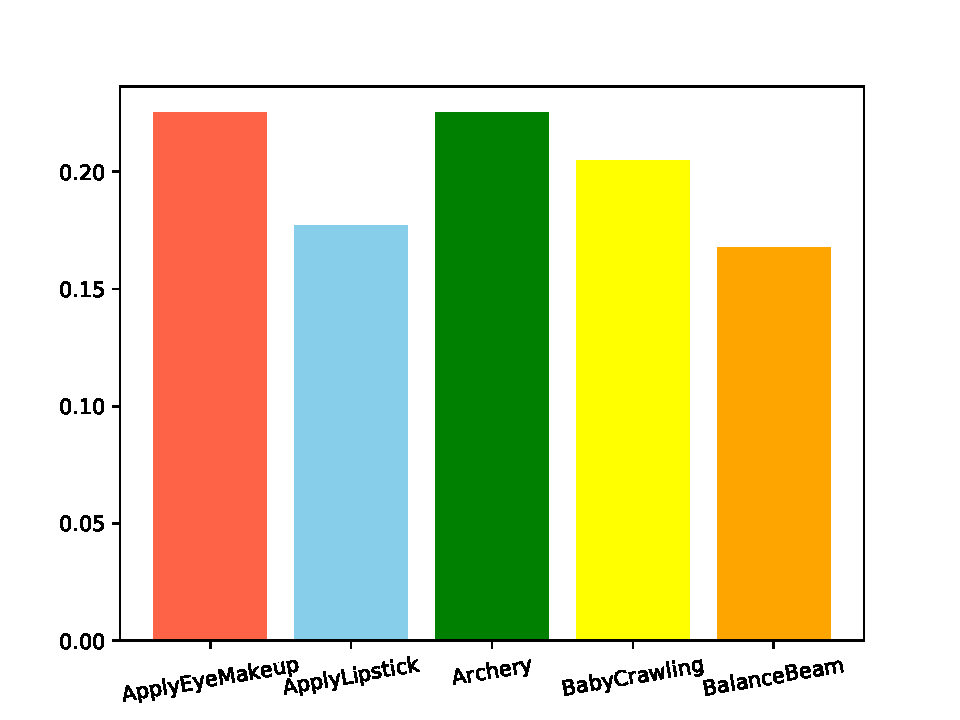
\includegraphics[scale=0.55]{Figures/histogram_5.pdf}
    \caption{Histogram of number of examples per class in UCF5.}
    \label{fig:hist_5}
\end{figure}

For the later experiments, we used the first \(10,15\) and \(20\) classes respectively, taken in an alphabetical order from the complete dataset. Also, with respect to the train and test partitions, they were created using the scripts provided for this assignment. These scripts divide the data in train and test (script \mintinline{bash}{1_move_files.py}) using  pre-made train and test lists created in the documentation of the dataset. Also, all the videos are divided in frames and stored in train and test folders automatically using the script \mintinline{bash}{2_extract_files.py}.

%%%%%%%%%%%%%%%%%%%%%%%%%%%%%%%%%%%%%%%%%%%%%%%%%%%%%%%%%%%%%%%%%%%%%%%%%%%%%%%%
\section{RESULTS AND ANALYSIS}
\label{section:results}
\subsection{5-classes experiments}

In order to test the fixed and random class models we repeated the validation process $20$ times. Table \ref{tab:results1} shows the min, max, mean and standard deviation of the accuracy for both models.

\begin{table}[H]
\centering
    \begin{tabular}{l|rrrr}
                     & min & max    & mean   & std    \\ \hline
    Fixed mode acc  & 0.2252       & 0.2252 & 0.2252 & 0.0000 \\
    Random mode acc & 0.1832     & 0.2376 & \textbf{0.2048} & 0.0156
    \end{tabular}
    \caption{Results of the dummiest models.}
    \label{tab:results1}
\end{table}

We can see how the fixed-class model's accuracy doesn't change over iterations, as expected. For these experiments, the first class is fixed for the mixed model. That is why the accuracy matches the ratio of elements in the first class over the whole dataset.

On the other hand, the random accuracy is not as consistent, and the obtained mean is quite close to the expected value, $1/5$, since there are $5$ classes in our dataset. Both results matches our theorical analysis.

\begin{figure}[H]
    \centering
    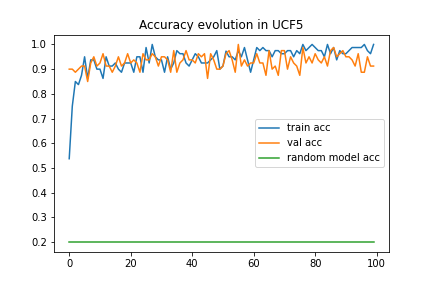
\includegraphics[scale=0.6]{Figures/inception-5-5.png}
    \caption{Train and validation accuracy curves of the CNN framework in the UCF5 dataset, compared to the dummy models.}
    \label{fig:UCF5:acc}
\end{figure}

Figure \ref{fig:UCF5:acc} shows the comparison of the frame-by-frame framework with the previous models. The CNN model clearly outperforms the random model, which was expected. With respect to the CNN framework results, we can say that the model achieves a really good accuracy score in about \(15\) epochs and then the improvement is not very impressive. Following our intuition, the model should Early Stop. In fact, we checked that the model has a \mintinline{bash}{CallBack} with the early stopping with a period of \(10\) epochs. However, we state that the oscilations of the learning curves (the loss function can be observed in Figures \ref{fig:train:loss} \ref{fig:val:loss}) lead to avoid the early stop. 

\begin{table}[H]
\centering
    \begin{tabular}{lr}
    Model          &    Accuracy    \\ \hline
    Fixed mode acc  & 0.2252  \\
    Random mode acc & 0.2048\\
    CNN &  \textbf{1.000}  \\
    \end{tabular}
    \caption{Comparison of the models used for UCF5.}
    \label{tab:results1:comp}
\end{table}

Table \ref{tab:results1:comp} depicts the comparison between the first two models and the CNN framework. We obtain a really odd result: the CNN method obtains the highest possible accuracy \(1.0\) in the train and validation set. This is an indicator that something is probably wrong. However, this is not a part of our developed code and we could not quickly determine the exact reason of this result.
    
\subsection{Complexity evolution with more classes}

The following goal is to increment the number of classes gradually and compare how the model performs with this class increment. A priori our model should decrease its performance when the number of classes increases since the problem becomes harder to solve, so it is harder for the models to generalize.

Figures \ref{fig:train:acc}, \ref{fig:val:acc} show that our previous statement is true. As we can see, the model that consider the lesser number of classes, called UCF5, achieves the highest accuracy values in each of the epochs. Also, each increment of the number of classes leads to a small decrease in the accuracy values, being the model that considers 20 classes (UCF20) the one with the lowest results in terms of accuracy.

\begin{figure}[]
    \centering
    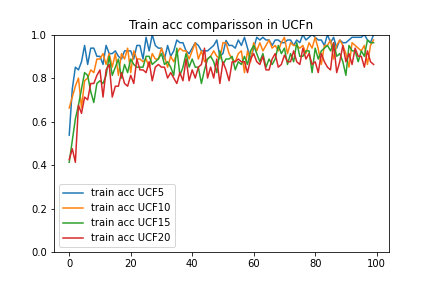
\includegraphics[scale=0.6]{Figures/UCF_train_acc_comparisson.png}
    \caption{Accuracy of the different models in the train set.}
    \label{fig:train:acc}
\end{figure}

\begin{figure}[]
    \centering
    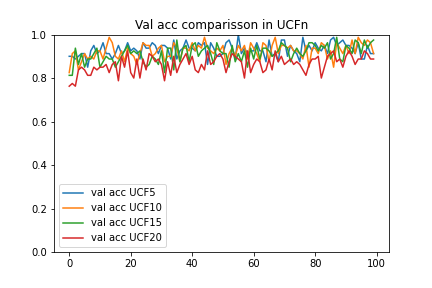
\includegraphics[scale=0.6]{Figures/UCF_val_acc_comparisson.png}
    \caption{Accuracy of the different models in the validation set.}
    \label{fig:val:acc}
\end{figure}

Figures \ref{fig:train:loss} and \ref{fig:val:loss} show the exact same behaviour when we consider the loss function. The higher the number of classes considered, the higher loss values obtained.

\begin{figure}[]
    \centering
    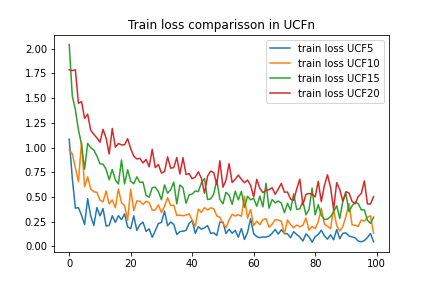
\includegraphics[scale=0.6]{Figures/UCF_train_loss_comparisson.png}
    \caption{Loss of the different models in the train set.}
    \label{fig:train:loss}
\end{figure}

\begin{figure}[]
    \centering
    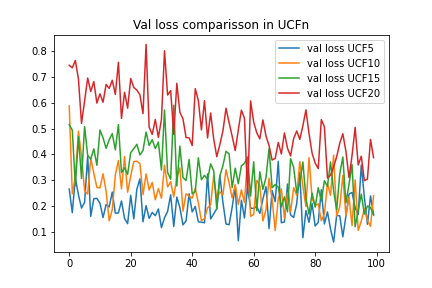
\includegraphics[scale=0.6]{Figures/UCF_val_loss_comparisson.png}
    \caption{Loss of the different models in the validation set.}
    \label{fig:val:loss}
\end{figure}

Additionally and although we do not specifically show any data we detected that the training time slightly increases when incrementing the number of classes.

Finally, table \ref{tab:results2} summarizes the results obtained for each of the different number of classes. These results match the previous analysis. It is remarkable the very high accuracy that this method obtains then the number of classes is as limited as ours. It could be studied if, in this case, the accuracy decreases linearly with the number of classes.

\begin{table}[H]
    \begin{tabular}{l|rrrr}
          & max train acc & max val acc & min train loss & min val loss \\ \hline
    UCF5  & 1.0000      & 1.0000 & 0.0439         & 0.0593       \\
    UCF10 & 0.9875        & 0.9875      & 0.1279         & 0.1042       \\
    UCF15 & 0.9750        & 0.9875      & 0.2339         & 0.1190       \\
    UCF20 & 0.9625        & 0.9250      & 0.3759         & 0.2504      
    \end{tabular}
    \caption{Results of the different UCFn models.}
    \label{tab:results2}
\end{table}

We have also noticed that all the values obtained are multiples of $0.005 = 1/200$, which is precisely the inverse of the batch size. Because of this, our current hypothesis is that the average accuracy is computed per batch instead of per epoch but we haven't been able to confirm nor deny such hypothesis. It is worth mentioning that we have not modified that part of the code.

%%%%%%%%%%%%%%%%%%%%%%%%%%%%%%%%%%%%%%%%%%%%%%%%%%%%%%%%%%%%%%%%%%%%%%%%%%%%%%%%
\section{CONCLUSIONS}
\label{section:conclusions}

In this practical assigment we have tackled the \textbf{action recognition task}, using one of the most important datasets for this problem with very advanced and complex (and not so complex) methods. These models perform really well when the number of classes is limited, and struggle generalizing when the number of classes increases. This behaviour depicts that for the whole dataset (101 classes) we might need state-of-the-art models such as transformers \cite{TRANSFORMERS}.

Despite the problems with Google Colab during the experiments of this assigment, we have learned a lot and genuently enjoy this practical assigment.

%%%%%%%%%%%%%%%%%%%%%%%%%%%%%%%%%%%%%%%%%%%%%%%%%%%%%%%%%%%%%%%%%%%%%%%%%%%%%%%%
\section{TIME LOG}
\label{section:timelog}
This practical assignment was fulfilled over the course of two full days, where both members of the team worked (literally) side by side with the following time log:

\begin{itemize}
    \item Theorical analysis: 2h.
    \item Implementing the models: 1h.
    \item Making the third model work on Colab: 10h.
    \item Executing the experiments: 2h.
    \item Analyzing and explained the results: 2h.
    \item Writing the final report: 8h.
\end{itemize}

The model trainings was parallelized with the report writing due to the long exeution times.

\printbibliography

\end{document}